\chapter{Preliminary concepts}

\section{The central dogma of molecular biology}

The central dogma explains how genetic information flows within a living being. It states that DNA, the molecule that stores the genetic information, is replicated by the enzyme DNA Polymerase. Also, RNA Polymerase produces messenger RNA (mRNA) from DNA in a process called transcription. Finally, the ribosomes read the sequence of the mRNA while they bind aminoacids to build the proteins. This process is called translation because ribosomes use a genetic code to translate from the language of nucleotides, the structural blocks of DNA and RNA, to the language of aminoacids, the structural blocks of proteins. \cite{alberts13}. Fig. \ref{fig:con-dogma} summarizes the central dogma.

In prokaryotes, DNA molecules exist in the form of chromosomes and plasmids. The former are the main genetic material that has the essential information to make the organisms. Prokaryotes have only a single copy of it, while eukaryotes may have several (e.g. we have $23$ pairs). The latter are shorter molecules that confer additional characteristics such as antibiotic resistance. There could be several copies in a cell and they can be transferred between organisms. Plasmids are extensively used in synthetic biology because they are easier to introduce in cells.

Proteins are the structural and functional elementary units of living beings. Therefore, according to the proteins that are being produced in a certain cell it will have certain form and develop certain functions. 

\begin{figure}[H]
  \centering
  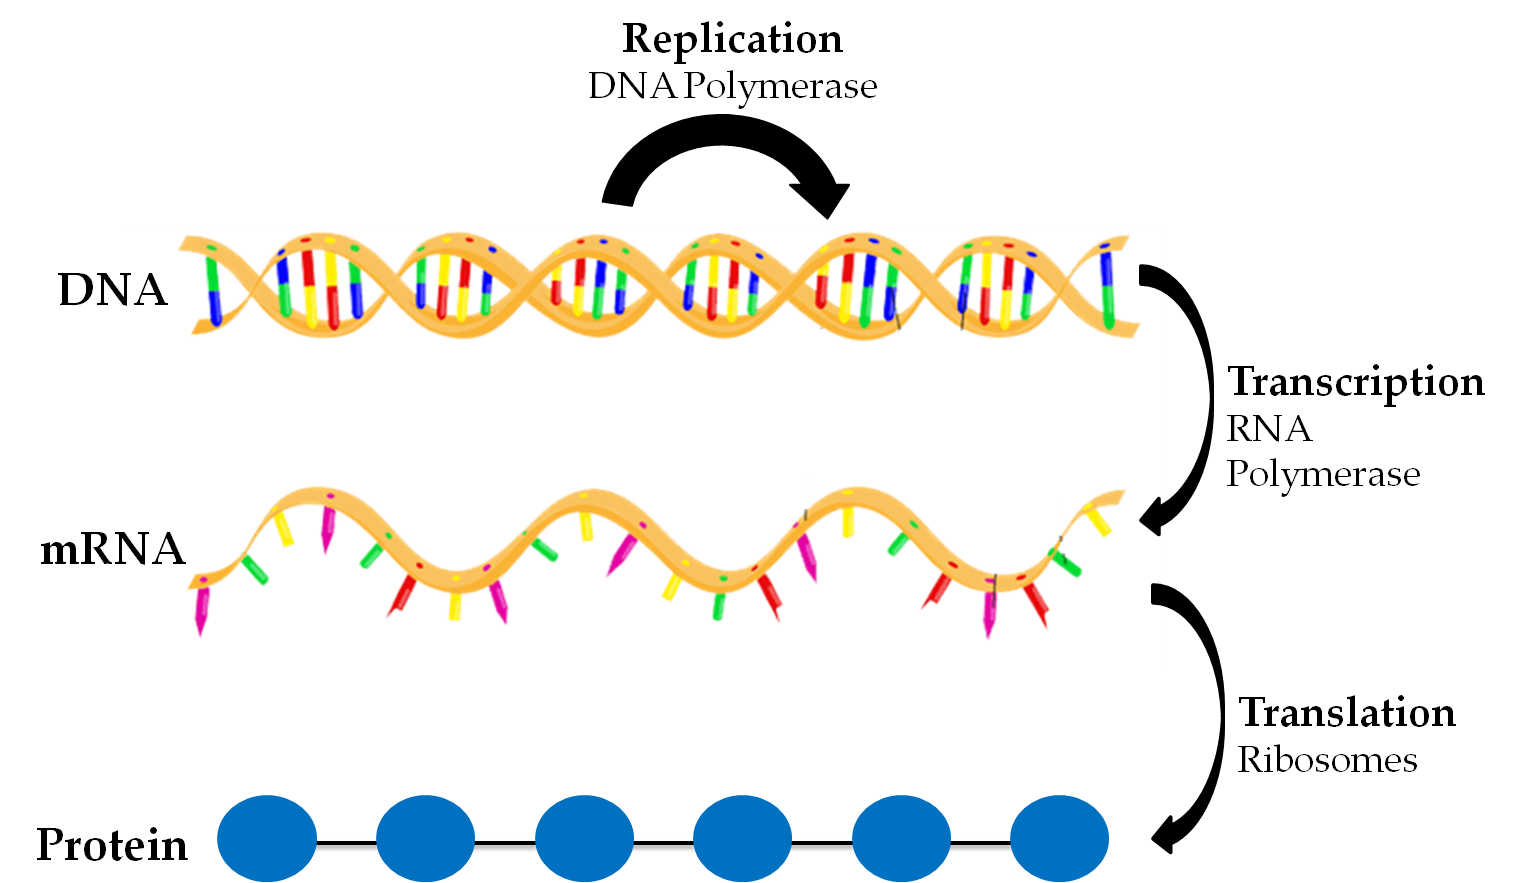
\includegraphics[width=15cm]{con-dogma}
  \caption[The central dogma of molecular biology]{\label{fig:con-dogma} The central dogma of molecular biology.}
\end{figure}

The encoding of information in DNA and the mechanisms by which proteins are made according to that information, including the genetic code, are very similar between different organisms. In eukaryotes, for instance there are more sophisticated processes of gene expression and regulation, but the mechanisms in general are the same for every living being. This remarkable fact supports the idea of a common ancestor for all the living beings and makes it possible, for instance, to use genes from different organisms to build synthetic biological circuits.

\section{Gene regulation and biological circuits}

DNA contains all the information necessary to build a living being and let him develop his functions. However, genetically identical cells may differ a lot. For example, our neurons are very different in form and function than our skin cells, even though they have the same genetic information. This differentiation happens because they are expressing different sets of genes at different levels. Moreover, cells are not static, they are constantly interacting with their surroundings and adjusting their gene expression according to the environment. To perform these functions, living beings have several mechanisms that allow them to regulate the rate of expression of their genes.

The genetic information encoded in the DNA is called genotype, while the observable characteristics of an organism are called phenotype. In this terminology, our neurons and our skin cells have the same genotype but differ in their genotypes \cite{alberts13} \cite{alon06}.

For each gene, or group of genes, there is a region located upstream the sequence that encodes for the protein called the promoter. mRNA Polymerase binds the promoter to initiate transcription. Also, there are proteins, called transcription factors (TFs), that bind specific sites in the promoter changing the rate of transcription. They may be either repressors or activators. The former reduce the transcription rate, while the latter increase it. Fig. \ref{fig:con-tf_simple} shows how the expression of some gene is enhanced by activators. Repressors also bind to the promoter but they lower the affinity between it and the RNApol, or actively obstruct the RNApol from binding to the DNA. There are promoters that are not regulated by any TF, they are called constitutive promoters.

\begin{figure}[H]
  \centering
  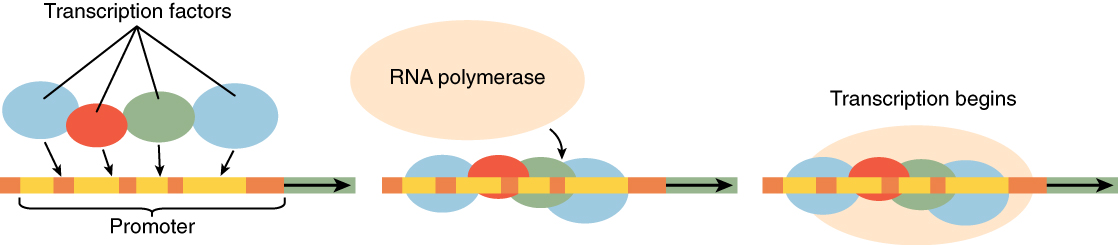
\includegraphics[width=12cm]{con-tf_simple}
  \caption[Scheme of transcriptional activation]{\label{fig:con-tf_simple} Scheme of transcriptional activation. (A) Transcription factors bind to specific regions in the promoter. (B) When the activators bind the promoter, they increase the affinity between the RNA Polymerase and the promoter. (C) Then, transcription starts more easily when the activators are bound to the promoter.}
\end{figure}


The mechanisms of gene regulation can be very complex. For example, a protein can inhibit the transcription of certain gene only when another molecule is bound to it. These molecules are called inducers and they are in some cases environmental signals. This is how gene expression responds to the surroundings of the cell. Besides, since TFs are proteins, they are codified by genes whose expression is controlled by other TFs and so on. In this way, different genes are connected between them and with the environment to allow the cells to take decisions in many sophisticated ways.

This is the principle of biological circuits, which are groups of genes and external signals that are connected by mechanisms such as the explained above, and develop some function in the cell. The approach to biological circuits that Systems Biology proposes is based on focusing on the interactions between the different genes and components from a quantitative point of view, rather than on specific details about the chemistry of the molecules involved. To illustrate this point, fig. \ref{fig:con-biocircuits_conv} shows some of the conventions used in Systems Biology to represent biological circuits. Synthetic circuits are usually simple, but natural circuits may be very complex, for instance, fig. \ref{fig:con-biocircuits_comp} shows a scheme of the circuit that controls the decision between the lytic and lysogenic pathways in lambda phage.

\begin{figure}[H]
  \centering
  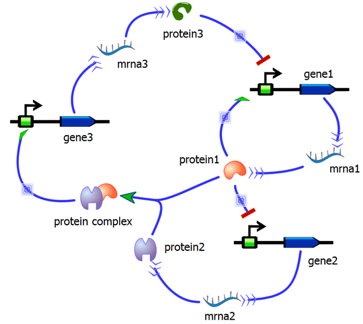
\includegraphics[width=13cm]{con-biocircuits_conv}
  \caption[Conventions used to represent biological circuits]{\label{fig:con-biocircuits_conv} Typical conventions used to represent biological circuits in Systems Biology. The lines are segments of DNA. $P_1$-$P_3$ are promoters, $A-D$ represent coding regions of the genes, the RBS (ribosome binding sites) are the sequences that bind the ribosome to start translation in the mRNA, and the regions labeled as Ter. are called transcriptional terminators and mark the end of transcription. In this case, $P_1$ is a constitutive promoter, protein $A$ represses the promoter $P_3$ and its repressing effect is in turn inhibited by the inductor $S_1$. Also, protein $C$ inhibits $P_2$ and thus the expression of its own gene, this is called negative autorregulation.}
\end{figure}

\begin{figure}[H]
  \centering
  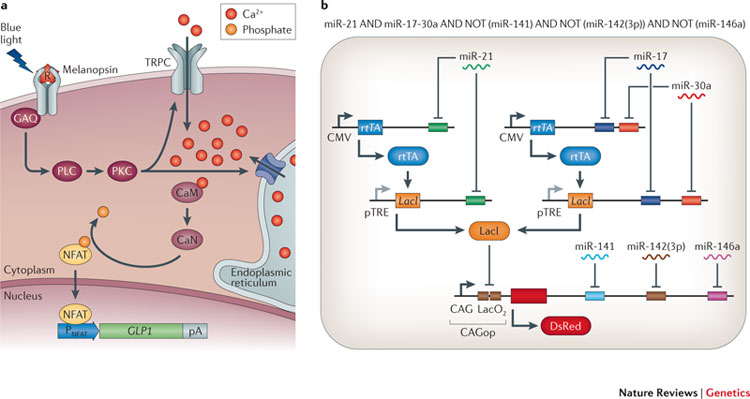
\includegraphics[width=12cm]{con-biocircuits_comp}
  \caption[Example of a biological circuit]{\label{fig:con-biocircuits_comp} Biological circuit that regulates the decision between lytic and lysogenic pathways in the life cycle of phage lambda. The scheme shows the complexity of natural genetic circuits.}
\end{figure}

In scheme such as the shown in fig. \ref{fig:con-biocircuits_conv}, the interacting components and the kind of interactions may be represented. However, to completely characterize these interactions, their strenghts must be given. A widely used model to quantify the strenght of gene regulation is the Hill equation.

\section{Hill functions}
\label{sec:hill}

To model the regulation on a gene by a transcription factor, a widely used model is the Hill equation. We will derive it for a simple case that gives an intuitive understanding of the basic principles \cite{alon06}.

Consider a transcription factor $X$ that binds to the promoter of some gene, we will label the promoter (gene) as $D$. Also, suppose that $X$ can bind to $n$ sites in the promoter and ignore the intermediate states where less than $n$ molecules of $X$ are bound. The chemical equation is

\begin{equation*}
  \ce{n[X] + [D]} \ce{<=>[k_+][k_-]} \ce{[nXD]}.
\end{equation*}

Hence, $[nXD]$ changes over time as

\begin{equation*}
  \frac{\mathrm{d}[nXD]}{\mathrm{d}t} = k_+[X]^n[D] - k_-[nXD],
\end{equation*}

which in steady state yields

\begin{equation}
  \label{eq:hillss}
  [X]^n[D] = \frac{k_-}{k_+}[nXD].
\end{equation}

Taking the total number $D_T$ of copies of the gene as a constant we obtain

\begin{equation*}
  [D_T] = [D]+[nXD].
\end{equation*}

Solving for the free DNA concentration $[D]$ and replacing in eq. \eqref{eq:hillss}

\begin{equation*}
  [X]^n\left([D_T]-[nXD]\right) = \frac{k_-}{k_+}[nXD].
\end{equation*}

$[nXD]/[D_T]$ and $[D]/[D_T]$ are the fractions of DNA bound and unbound to the transcription factor, respectively, solving for these quantities we obtain

\begin{equation*}
  \frac{[nXD]}{[D_T]} = \frac{[X]^n}{K_d^n+[X]^n}, \quad\quad\quad\quad\quad  \frac{[D]}{[D_T]} = \frac{K_d^n}{K_d^n+[X]^n} = \frac{1}{1+\left(\frac{[X]}{K_d}\right)^n},
\end{equation*}

where $K_d^n \coloneqq k_-/k_+$. In a timescale such that many bindings and unbindings of the transcription factor to the promoter have occurred, the fractions can be interpreted as the probability for the promoter to be bound to $n$ molecules of $X$ and unbound, respectively. If we assume that the increment in the transcription rate with respect to the basal rate $a$ is proportional to the probabilities of being bound for an activator, and of being unbound for a repressor, the net rates are

\begin{equation}
  \label{eq:con-hillac}
  f([X]) = a + b \frac{[X]^n}{K_d^n+[X]^n},
\end{equation}

for an activator, and

\begin{equation}
  \label{eq:con-hillrep}
  f([X]) = a + b \frac{1}{1+\left(\frac{[X]}{K_d}\right)^n}.
\end{equation}

for a repressor. $b+a$ is the maximum transcription rate, wich happens when $[X]\rightarrow\infty$ for the case of an activator, and when $[X]=0$ for the repressor. $K_d$ is called the dissociation constant, which is the concentration of $X$ needed for half activation or repression. Biologically it represents the chemical affinity between $X$ and the promoter. $n$ is called the Hill coefficient and it is related to the cooperativity of the transcription factor. It is large if the binding of a molecule of $X$ enhances the binding of another one and this results in a more step-like Hill function. Figures \ref{fig:con-hill_act} and \ref{fig:con-hill_rep} show a typical Hill curve.

\begin{figure}[H]
  \centering
  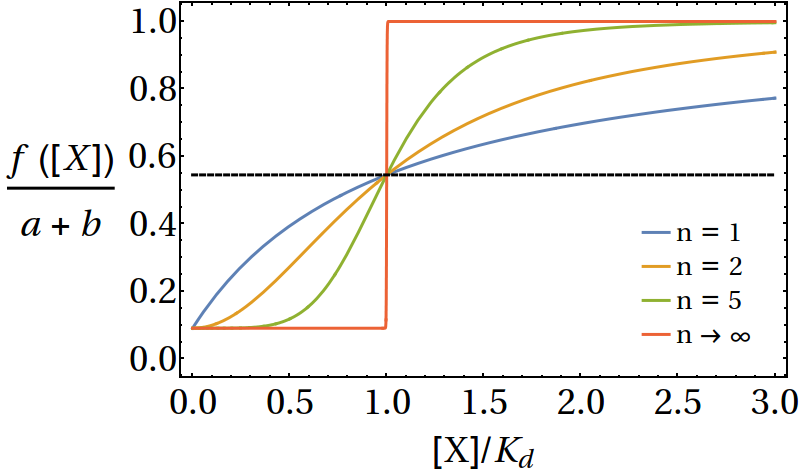
\includegraphics[width=14cm]{con-hill_act}
  \caption[Hill functions for an activator]{\label{fig:con-hill_act} Hill functions for an activator given by eq. \eqref{eq:con-hillac}. Various values of $n$ are shown. The dashed line shows the point of half activation corresponding to $[X]=K_d$. All have the same value of $K_d$, $a$ and $b$ with $b/a=10$.}
\end{figure}

\begin{figure}[H]
  \centering
  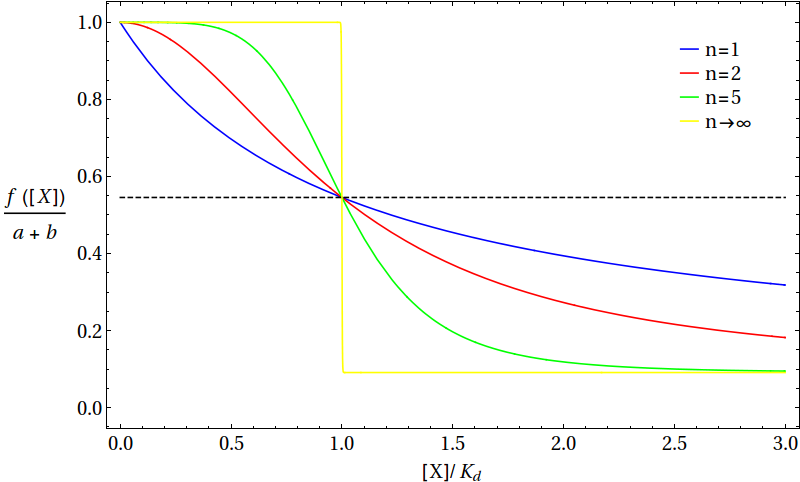
\includegraphics[width=14cm]{con-hill_rep}
  \caption[Hill functions for a repressor]{\label{fig:con-hill_rep} Hill functions for a repressor given by eq. \eqref{eq:con-hillrep}. The same parameters as in fig. \ref{fig:con-hill_act} are used.}
\end{figure}

Notice in both graphs that as $n\rightarrow\infty$, the function approaches a Heaviside function with the step in $[X] = K_d$. This approximation is useful on a first qualitative analysis of biological circuits but such high values of $n$ are biologically unrealistic. The case $n=1$ corresponds to the Michaelis-Menten equation \cite{alon06}.

\section{Probability}

Consider an experiment in which the set of possible outcomes is known. A random variable $X$ is a quantity that can take values from that set of possible outcomes $\{x\}$ of the experiment. How likely is that any value $x$ happens in a given trial of the experiment is determined by the probability mass function (PMF) $P(x)$ if the variable is discrete. $P(x)$ represents the fraction of trials of the experiment in which $X$ has the value $x$ when the number of trials is large. The PMFs follow the axioms of nonnegativity, additivity and normalization \cite{bertsekas08} \footnote{We will focus here on discrete random variables. The continous case is very similar, it reduces almost entirely to change $\sum$ by $\int\mathrm{d}x$ and $P(x)$ by $\rho(x)$, where $\rho(x)$ is the probability density function (PDF), the analogous of the PMF.}.

For several random variables $X_1,\dotsc,X_n$, the joint PMF  $P(x_1,\dotsc,x_n)$ is defined as the probability that $X_1=x_1,\dotsc,X_n=x_n$. The set of random variables are \textbf{independent} if

\begin{equation*}
  P(x_1,\dotsc,x_n) = P(x_1)\dotsm P(x_n)
\end{equation*}

The conditional probability of the random variables $X_1,\dotsc,X_k$ given the variables $X_{k+1},\dotsc,X_n$ is denoted by $P(x_1,\dotsc,x_k|x_{k+1},\dotsc,x_n)$ and it is defined as

\begin{equation*}
  P(x_1,\dotsc,x_k|x_{k+1},\dotsc,x_n) \coloneqq \frac{P(x_1,\dotsc,x_n)}{P(x_{k+1},\dotsc,x_n)},
\end{equation*}

provided that the denominator is different from $0$. It can be thought as the probability of a certain outcome for $X_1,\dotsc,X_k$ when certain given values for $X_{k+1},\dotsc,X_n$ have been obtained. Notice that if all the random variables are independent it reduces to

\begin{equation*}
  P(x_1,\dotsc,x_k|x_{k+1},\dotsc,x_n) = P(x_1,\dotsc,x_k).
\end{equation*}

The conditional and unconditional probabilities are equal, meaning that the outcome of $(X_{k+1},\dotsc,X_n)$ does not affect the outcome of $(X_1,\dotsc,X_k)$.

To find the probability of a certain outcome of $X$, sometimes it is easier to use the \textbf{total probability theorem}

\begin{equation*}
  P(x) = \sum_y P(x,y) = \sum_y P(x|y)P(y).
\end{equation*}

The \textbf{expected value} (also called mean or average) of a function of a random variable $f(X)$ is defined as

\begin{equation}
  \label{eq:con-ave_def}
  \langle f(X)\rangle \coloneqq \sum_xf(x)P(x).
\end{equation}

From the definition can be noticed that the expected value is linear, i.e., for a pair of random variables $X$ and $Y$, and a constant $c$

\begin{equation*}
  \langle X+cY\rangle = \langle X\rangle+c\langle Y\rangle.
\end{equation*}

The variance $\sigma^2(X)$ of $X$ measures the dispersion of the possible outcomes of the random variable, it is defined as

\begin{equation*}
  \sigma^2(X) \coloneqq \left\langle\left( X-\langle X\rangle\right)^2\right\rangle.
\end{equation*}

It can be easily shown that

\begin{equation}
  \label{eq:con-var_nice}
  \sigma^2(X) = \langle X^2\rangle - \langle X\rangle^2.
\end{equation}

For a constant $c$, the variance has the property

\begin{equation*}
  %\label{eq:con-var_const}
  \sigma^2(cX) = c^2\sigma^2(X)
\end{equation*}

The $\mathbf{n}$\textbf{th moment} of the random variable $X$ is given by

\begin{equation*}
  \langle X^n\rangle \coloneqq \sum_xx^nP(x).
\end{equation*}

Hence, the expected value is the first moment and the variance can be written in terms of the first and second moments.

If $X$ and $Y$ are independent,

\begin{equation}
  \label {eq:con-mom_ind}
  \langle XY\rangle = \langle X\rangle\langle Y\rangle \quad\text{and}\quad \sigma^2(X+Y) = \sigma^2(X)+\sigma^2(Y).
\end{equation}

The conditional expectation of $X$ given a random variable $Y$, $\langle X|Y\rangle$ is itself a random variable which depends on $Y$. When $Y$ is fixed in some $y$ it is given by

\begin{equation*}
  \langle X|y\rangle \coloneqq \sum_xxP(x|y),
\end{equation*}

and it follows that

\begin{equation*}
  %\label{eq:con-total_exp}
  \left\langle\langle X|Y\rangle\right\rangle = \left\langle X\right\rangle
\end{equation*}

which is the \textbf{law of total expectation}, for the variance there is an analogous theorem called the \textbf{law of total variance}

\begin{equation*}
  \label{eq:con-total_var}
  \sigma^2(x) = \left\langle\sigma^2(x|y)\right\rangle + \sigma^2\left(\langle x|y\rangle\right).
\end{equation*}

The \textbf{covariance} of $X$ and $Y$ is defined as

\begin{equation*}
  \text{cov}(X,Y) \coloneqq \left\langle\left(X-\langle X\rangle\right)\left(Y-\langle Y\rangle\right)\right\rangle = \langle XY\rangle - \langle X\rangle\langle Y\rangle.
\end{equation*}

It is as a measure of how correlated is the behaviour of $X$ and $Y$. For example, if the value of $Y$ is known, the value of $X$ will be more likely to be known if the covariance is high in absolute value. The covariance will be $0$ if it does not give us any information. Consider the extreme cases, if $Y=X$, $\text{cov}(X,X) = \sigma^2(X)$, while if $X$ and $Y$ are independent, from eq. \eqref{eq:con-mom_ind} we get $\text{cov}(X,Y) = 0$.

\section{Noise}
\label{sec:con-noise}
Intuitively, we may expect that a random variable is more ``random'' or noisy when its deviations relative to its expected value are larger. With this in mind, the noise in a random variable $X$ must increase as the variance increases and decrease as the mean increases (the same deviation from a smaller expected value is more notorious than from a larger one). The quantities that have benn used to measure noise in biology are the Fano factor $\nu$ and the coefficient of variation (CV) $\eta$, which are defined by

\begin{equation}
  \label{eq:con-fano_def}
  \nu_X \coloneqq \frac{\sigma^2(X)}{\langle X \rangle},\quad\quad\eta_X \coloneqq \frac{\sigma(X)}{\langle X \rangle}.
\end{equation}

The Fano factor has been used in the first studies of noise in biology because it measures the deviations from a Poissonian behavior. For a random variable with a Poisson PMF, $\nu_X=1$. In more recent studies the coefficient of variation is being used because it is dimensionless, so it does not depend on the units that are used. For this reason, the generic term 'noise' is now used refering to $\eta$.

\section{Moment generating functions}

Let $n_1,\dotsc,n_N$ be discrete random variables over $\mathbb{N}$ and let $f(n_1,\dotsc,n_N)$ be their joint PMF. The moment generating function $F(z_1,\dotsc,z_N)$ is defined as

\begin{equation}
  \label{def:mom_gen}
  F(z_1,\dotsc,z_N) \coloneqq \sum_{\mathclap{n_1=0}}^{\infty} \dotsi \sum_{\mathclap{n_N=0}}^{\infty} z_1^{n_1} \dotsm z_N^{n_N} f(n_1,\dotsc,n_N).
\end{equation}

Evaluating the function at $z_1 = \dotsb = z_N = 1$ (denoted by $\left. \right|_1$)

\begin{equation}
  \label{eq:con-mom_gen_1}
  \left.F\right|_1 = \sum_{\mathclap{n_1,\dotsc,n_N}}f(n_1,\dotsc,n_N) = 1
\end{equation}

by the axiom of normalization. Taking the derivative of eq. \eqref{def:mom_gen} with respect to $z_i$, $i = 1,\dotsc,N$ we get

\begin{equation}
  \label{eq:con-mom_gen_d1}
  \left.\frac{\partial F}{\partial z_i}\right|_1 = \left.\sum_{\mathclap{n_1,\dotsc,n_N}}n_i z_1^{n_1}\dotsm z_i^{n_i-1}\dotsm z_N^{n^N}f(n_1,\dotsc,n_N)\right|_1 = \sum_{\mathclap{n_1,\dotsc,n_N}} n_i f(n_1,\dotsc,n_N) = \langle n_i \rangle.
\end{equation}

Differentiating again with respect to $z_j$, $j=1,\dotsc,N$ with $j\neq i$

\begin{equation}
  \label{eq:con-mom_gen_d1d2}
  \left. \frac{\partial F}{\partial z_i z_j} \right|_1 = \langle n_i n_j \rangle.
\end{equation}

Differentiating eq. \eqref{def:mom_gen} twice with respect to $z_i$ we obtain similarly

\begin{equation}
  \label{eq:con-mom_gen_d1d1}
  \left. \frac{\partial^2F}{\partial z_i^2}\right|_1 = \langle n_i(n_i-1) \rangle.
\end{equation}

These properties will be very useful in the next sections to find the noise of a genetic system.

\section{Characteristic function}
\label{sec:con-charac_func}
Another quantity that is used to find the moments of a random variable is the characteristic function. For a $N$-tuple of random variables $(X_1,\dotsc,X_N)$ with PMF $f$, it is defined as

\begin{equation*}
  \phi(s_1,\dotsc,s_N)\coloneqq \left\langle e^{\sum_{i=1}^Ns_ix_i}\right\rangle = \sum_{x_1}\dotsi\sum_{x_N}\exp\left(\sum_{i=1}^Ns_ix_i\right)f(x_1,\dotsc,x_N).
\end{equation*}

Denote the evaluation at $s_1=\dotsb=s_N=0$ by $|_0$. From the axiom of normalization

\begin{equation*}
  \phi(s)|_0 = 1.
\end{equation*}

Differentiating once with respect to $s_i$ for $i=1,\dotsc,N$.

\begin{equation*}
  %\label{eq:con-char_1}
  \left.\frac{\partial\phi(s_1,\dotsc,s_N)}{\partial s_i}\right|_0 = \left.\left\langle x_i e^{\sum_{i=1}^Ns_ix_i}\right\rangle\right|_0 = \langle x_i\rangle.
\end{equation*}

Each differentiation with respect to $s_i$ produces a factor $x_i$ in the average, hence

\begin{equation*}
  %\label{eq:con-char_2}
  \left.\frac{\partial^2\phi(s_1,\dotsc,s_N)}{\partial s_i \partial s_j}\right|_0 = \langle x_ix_j\rangle.
\end{equation*}

This equation is valid for any $i,j=1,\dotsc,N$, even for the case $i=j$. In that case the right hand side becomes $\langle x_i^2\rangle$. By calculating higher order derivatives higher order moments can be found.
  
\section{Stochastic processes}

A stochastic process $X(t)$\footnote{or $\{X\}_n$ if the time steps are discrete} is a set of random variables indexed by another variable, which in many cases is the time. An outcome of the stochastic process is a function of time which varies randomly between different repetitions of the experiment \cite{vankampen92} \cite{gardiner03}.

The \textbf{autocorrelation} $C_X$ of a stochastic process $X(t)$ is given by

\begin{equation*}
  C_X(t,t') \coloneqq \langle X(t)X(t')\rangle.
\end{equation*}

It measures the degree of correlation between outcomes of the random variables at different times. If the process $X(t)$ is \textbf{stationary}, the autocorrelation only depends on the time difference, i.e.

\begin{equation*}
  C_X(\tau) \coloneqq \langle X(t)X(t+\tau)\rangle,
\end{equation*}

where $\tau \coloneqq t'-t$.

The \textbf{power spectrum} $S_X$ of a stochastic process is defined as average of the square norm of its the Fourier transform, i.e.

\begin{equation*}
  S_X(\omega) \coloneqq \left|\langle\hat X\rangle\right|^2.
\end{equation*}

The Fourier transform and the power spectrum are related by the \textbf{Wiener-Khinchin theorem}. It states that the power spectrum and the autocorrelation are Fourier-Transform pairs, i.e.

\begin{equation}
  \label{eq:con-wkth}
  \mathscr{F}(C_X(\tau)) = S_X(\omega),\quad\text{and}\quad \mathscr{F}^{-1}(S_X(\omega)) = C_X(\tau).
\end{equation}

\section{The Poisson process}
\label{sec:poisson}

The processes of creation and destruction involving gene expression are usually modeled as Poisson processes. For example, the creation and destruction of mRNA molecules and proteins. The Poisson process is a continous-time stochastic process that is used to model arrivals when there is some known arrival rate and when the arrivals at different time intervals are independent.

Mathematically, we define $P(k,\tau)$ as the probability that there are $k\in\mathbb{N}$ arrivals during a time interval $\tau$. Letting $\lambda$ be the arrival rate, the Poisson process satisfy the following properties

\begin{itemize}
  \item  $P(k,\tau)$ is the same for all intervals of length $\tau$.
  \item  The value of $P(k,\tau)$ during some particular interval is independent of other intervals.
  \item $P(k,\tau)$ satisfies the following
    \begin{equation*}
      \begin{split}
        P(0,\tau)=1-\lambda\tau+o_0(\tau),\\
        P(1,\tau)=\lambda\tau+o_1(\tau),\\
        P(k,\tau)=o_k(\tau).\quad\text{for } k>1.
      \end{split}
    \end{equation*}
    
    Where $o_k(\tau)$, $k=0,1,\dotsc$ are functions that become negligible compared to $\tau$ as it becomes small, i.e.

    \begin{equation*}
      \lim_{\tau\to 0}\frac{o_k(\tau)}{\tau}=0.
    \end{equation*}
\end{itemize}

According to the previous properties, $P(k,\tau)$ is given by

\begin{equation*}
  P(k,\tau) = e^{-\lambda\tau}\frac{(\lambda\tau)^k}{k!},\quad k=0,1,\dotsc
\end{equation*}

which is the Poisson PMF. Let $N_\tau$ be the number of arrivals during a time interval $\tau$. Then, using the definition for the expected value and variance [eqs. \eqref{eq:con-ave_def} and \eqref{eq:con-var_nice}] we get

\begin{equation*}
  \langle N_\tau\rangle = \sigma^2(N_\tau) = \lambda \tau.
\end{equation*}

The average number of arrivals in a time $\tau$ is, as one may expect, the arrival rate times the length of the interval. From eq. \eqref{eq:con-fano_def}, the noise and Fano factor for $N_\tau$ are

\begin{equation*}
  %\label{eq:con-poisson_noise}
  \nu(N_\tau) = 1,\quad\quad \eta(N_\tau) = \frac{1}{\sqrt{N_\tau}}.
\end{equation*}

If the number of arrivals is very large, the Poisson noise is negligible. However, for a biological system this is not always the case. For instance, the average number of copies of mRNA of a given gene is of the order of only $10$. Moreover, although the mean number of proteins is of the order of $1000$, their Poisson noise is very small. In spite of that, there is an important contribution of noise transmitted from mRNA and other sources as we will see in chapter \ref{ch:master}.

Now we find the PDF $f_T(t)$ for the time between events, by now let $t=0$ be the time at which the last event occured, and let $t=T$ the time until the next event, then

\begin{equation*}
  P(T\leq t) =\int_0^tf_T(t')dt'=1-P(T>t) = 1 - P(0,t) = 1 - e^{-\lambda t}.
\end{equation*}

Differentiating and applying the fundamental theorem of calculus, we get the \textbf{exponential PDF}, which is given by

\begin{equation}
  \label{eq:con-exp_pdf}
  f_T(t) = \lambda e^{-\lambda t}.
\end{equation}

The exponential PDF is \textbf{memoryless} in the following sense: suppose an arrival happened at time $t'$, then the probability distribution for the remaining time until the next arrival is an exponential with the same rate. With this in mind, not only the time until the first arrival, but all the interarrival times (the times between arrivals), follow the distribution given by eq. \eqref{eq:con-exp_pdf}.

Consider $k$ independent Poisson processes with rates $\lambda_1,\dotsc,\lambda_k$, and consider also a merged process in which an arrival is recorded each time an arrival occurs in either of the $k$ processes. The merged process is also Poissonian with rate $\Lambda\coloneqq\sum_{i=1}^k\lambda_i$. Besides, any arrival of the merged process has a probability $\lambda_i/\Lambda$, $i=1,\dotsc,k$ of corresponding to the $i$th process.

For the models explained in this work there might be several creation and destruction events which are Poissonian and independent, e.g. the synthesis and degradation of molecules, the binding of transcription factors, etc. Using the memorylessness and the merging properties of the Poisson process, precise and efficient simulations can be developed.

\section{The Gillespie algorithm}

To make simulations of the chemical equation that determine gene regulation we use the Gillespie algorithm \cite{gillespie77}. It is used to simulate simultaneous Poissonian events that occur with a certain rate (probability per unit time), e.g. synthesis and degradation of molecules, binding of an enzyme to a substrate, etc.

In the brute-force method we fix a time interval that must be sufficiently small. Then, for every possible event we sample a random number that according to the probabilities of the events, tells us which one occured. This procedure is repeated for all the intervals. Since time intervals must be small and for each interval we sample as many random numbers as events, this approach is very inefficient.

The Gillespie algorithm is by far more efficeint as it takes advantage of the merging and memorylessness properties of the Poisson process. A random number is sampled from an exponential distribution whose rate $\Lambda$ is the sum of the rates of the individual processes to find the time of occurence of the next event and another uniform one is sampled to evaluate which of the events occured. Using the properties of the exponential CDF, to obtain a number $X$ from an exponential distribution with parameter $\Lambda$ by sampling a number $U$ from an uniform distribution between $0$ and $1$ we apply the following equation

\begin{equation*}
  X = -\frac{1}{\Lambda}\ln(U).
\end{equation*}

The Gillespie algorithm is better than the brute-force method for several reasons. First, it does not defines a fixed small time interval, it finds the time intervals between events. Second, the number of random numbers sampled per time interval in the brute-force approach is equal to the number of events (which can be large), and many of the intervals there will not be an event, while in the Gillespie algorithm only two random numbers are sampled by event and the way in which the time interval is sampled allows to go forward in time in many fewer steps. Finally, a very important aspect to notice is that the Gillespie algorithm is exact, while the precision of the brute-force algorithm depends on how small is the time interval in consideration.
